% Promoted from L18; H9 gradient geometry retained. One website/handout source.
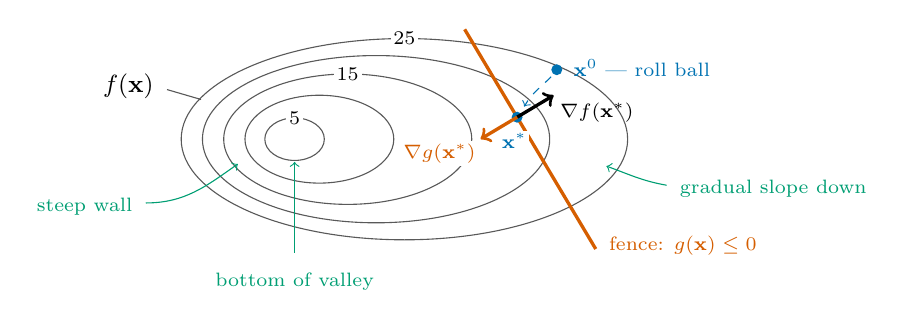
\begin{tikzpicture}[scale=0.90,every node/.style={font=\scriptsize}]
\definecolor{cifenceorange}{HTML}{D55E00}
\definecolor{cifenceblue}{HTML}{0072B2}
\definecolor{cifencegreen}{HTML}{009E73}
  % Valley contours: innermost at the far LEFT, elongated to the right, so the
  % wall is steep on the left and the slope is gradual on the right.
  \foreach \cx/\rx/\ry in {1.00/0.42/0.30, 1.35/1.05/0.62, 1.75/1.75/0.92,
                           2.15/2.45/1.18, 2.55/3.15/1.42}
    \draw[black!65] (\cx,1.8) ellipse ({\rx} and {\ry});
  \node[fill=white,inner sep=1pt] at (1.00,2.10) {5};
  \node[fill=white,inner sep=1pt] at (1.75,2.72) {15};
  \node[fill=white,inner sep=1pt] at (2.55,3.22) {25};
  \node[anchor=east,font=\small] at (-0.85,2.55) {$f(\mathbf{x})$};
  \draw[black!65] (-0.80,2.50) -- (-0.32,2.36);
  % green annotations
  \node[cifencegreen,anchor=east] at (-1.15,0.85) {steep wall};
  \draw[->,cifencegreen] (-1.10,0.90) to[out=0,in=215] (0.20,1.45);
  \node[cifencegreen,anchor=north] at (1.00,0.05) {bottom of valley};
  \draw[->,cifencegreen] (1.00,0.20) -- (1.00,1.48);
  \node[cifencegreen,anchor=west] at (6.30,1.10) {gradual slope down};
  \draw[->,cifencegreen] (6.25,1.15) to[out=170,in=340] (5.40,1.42);
  % the fence
  \draw[very thick,cifenceorange] (3.40,3.35) -- (5.25,0.25);
  \node[cifenceorange,anchor=west] at (5.30,0.30)
    {fence: $g(\mathbf{x}) \le 0$};
  % the ball: starts on the far side of the fence from the valley bottom
  \fill[cifenceblue] (4.70,2.78) circle (2.2pt);
  \node[cifenceblue,anchor=west] at (4.80,2.80)
    {$\mathbf{x}^0$ --- roll ball};
  \draw[->,cifenceblue,dashed] (4.62,2.68) to[out=225,in=60] (4.24,2.26);
  % x* = the TANGENCY point: the point of the fence on the lowest contour it
  % touches. Computed, not eyeballed -- see the geometry note below.
  \fill[cifenceblue] (4.14,2.11) circle (2.2pt);
  \node[cifenceblue,anchor=north,fill=white,inner sep=1pt] at (4.10,1.93)
    {$\mathbf{x}^*$};
  % Gradient arrows at x*: both along the fence normal +-(0.8587,0.5125), and
  % antiparallel to each other, which is what grad f + u grad g = 0 requires.
  \draw[->,very thick] (4.14,2.11) -- (4.655,2.418);
  \node[anchor=north west,inner sep=1pt] at (4.70,2.36)
    {$\nabla f(\mathbf{x}^*)$};
  \draw[->,very thick,cifenceorange] (4.14,2.11) -- (3.625,1.802);
  \node[cifenceorange,anchor=north east,fill=white,inner sep=1pt] at (3.60,1.78)
    {$\nabla g(\mathbf{x}^*)$};
\end{tikzpicture}
